% !LW recipe = latexmk (xelatex)
\documentclass[11pt,a4paper]{article}
\usepackage{fontspec}
\setmainfont{cmunrm.otf}[BoldFont=cmunbx.otf,ItalicFont=cmunti.otf,BoldItalicFont=cmunbi.otf]
\usepackage[english,russian]{babel}
\usepackage[margin=24mm,top=20mm,bottom=22mm]{geometry}
\usepackage{amsmath,amssymb,booktabs,graphicx,caption,microtype}
\usepackage[unicode,hidelinks]{hyperref}
\hypersetup{pdftitle={Спектральные нейрооператоры для задачи рассеяния при изменении волнового числа}}
\captionsetup{font=small,labelfont=bf,labelsep=period}
\setlength{\parindent}{1.25em}
\setlength{\emergencystretch}{1.2em}
\newcommand{\ii}{\mathrm{i}}
\newcommand{\R}{\mathbb R}
\newcommand{\C}{\mathbb C}
\newcommand{\T}{\mathsf T}
\newcommand{\norm}[1]{\lVert #1\rVert}
\newenvironment{localtable}{\par\medskip\begingroup\centering\small\renewcommand{\arraystretch}{1.18}}{\par\endgroup\medskip}
\newenvironment{localfigure}{\par\smallskip\begingroup\centering}{\par\endgroup\smallskip}
\makeatletter
\newcommand{\tabinput}[1]{\@@input #1.tex }
\makeatother
\begin{document}
\begin{center}{\Large\bfseries Сравнение спектральных нейрооператоров для задачи рассеяния при изменении материала и волнового числа\par}\end{center}
\noindent\textbf{Аннотация.}
Исследуется приближение комплексного рассеянного поля в среде с проницаемыми круговыми включениями. Материальные коэффициенты меняются в двух группах включений. На общей эталонной сетке решены 1\,240 задач при положительных волновых числах от $0{,}05$ до 4. Статическая задача при $k=0$ рассматривается отдельно. Сравниваются SVD-SNO, FNO и нейрооператоры с базисами Чебышёва и Фурье. Во всех четырёх случаях восстанавливается рассеянное поле, и погрешность измеряется в комплексной конечно-элементной норме $L^2$. \input{tables/abstract}

\smallskip\noindent\textbf{Ключевые слова:} уравнение Гельмгольца, метод конечных элементов, сингулярное разложение, спектральный нейрооператор, базис Фурье, полиномы Чебышёва.

\section*{Введение}
При изменении волнового числа меняются и характер пространственных колебаний, и величина рассеянного поля. Поэтому при сравнении нейрооператоров важно оценивать погрешность на каждой задаче относительно нормы её собственного решения. Общая сумма квадратов ошибок по выборке приписала бы больший вес полям с большой амплитудой.

Рассмотрим четыре способа построения отображения от параметров среды и падающей волны к решению. В SVD-SNO пространственные моды определяются по снимкам МКЭ. В двух вариантах спектрального нейрооператора Фанаскова и Оселедца используются заранее заданные функциональные базисы~\cite{fo}. В FNO преобразование Фурье задаёт линейную часть слоя, а нелинейность действует в пространственных узлах~\cite{li}. Цель работы состоит в том, чтобы сравнить точность этих представлений на одних и тех же новых средах при увеличении обучающей выборки с 400 до 1\,000 полей.

\section{Постановка задачи}
Пусть $\Omega=(-2,2)^2$. В группу $D_1$ входят 19 кругов радиусов $0{,}02$ и $0{,}05$, в группу $D_2$ входят пять кругов радиуса $0{,}10$. Тензор $A=aI$ изотропен. На $D_j$ заданы $a=a_j$ и $n=n_j$, в фоне оба скаляра равны единице. Вектор среды $p=(a_1,a_2,n_1,n_2)$ принадлежит прямоугольнику $[0{,}4;0{,}9]^2\times[2;6]^2$. Для падающей волны $u_i(x)=\exp(\ii k d\cdot x)$, $d=(\cos\theta,\sin\theta)$, требуется найти рассеянное поле $u_s$. Полное поле $u=u_i+u_s$ удовлетворяет
\begin{equation}
 \nabla\!\cdot(a\nabla u)+k^2nu=0\quad\text{в }\Omega,\qquad
 a\partial_\nu u_s-\ii ku_s=0\quad\text{на }\partial\Omega .
 \label{eq:wave}
\end{equation}
Через $\nu$ обозначена внешняя нормаль. На границах материалов непрерывны $u$ и нормальная компонента потока $a\nabla u$. Внешнее условие первого порядка приближённо описывает излучение.

\clearpage
\section{Метод конечных элементов и эталонная норма}
Введём пространство $V_h\subset H^1(\Omega;\C)$ непрерывных кусочно-линейных функций. Сетка согласована с границами включений и содержит 53\,246 узлов и 105\,690 треугольников. Материальные коэффициенты постоянны внутри каждого элемента. Подставляя $u_i+u_s$ в~\eqref{eq:wave} и интегрируя по частям, получим дискретную задачу: найти $u_h\in V_h$, для которого при всех $v\in V_h$
\begin{align}
 \int_\Omega a\nabla u_h\cdot\nabla\bar v
 - k^2\int_\Omega n u_h\bar v-\ii k\int_{\partial\Omega}u_h\bar v
 &=\int_\Omega(1-a)\nabla u_i\cdot\nabla\bar v
 +k^2\int_\Omega(n-1)u_i\bar v .
 \label{eq:weak}
\end{align}
Интегралы справа вычисляются по элементам с ненулевым контрастом. В матричном виде
\[
 (K_a-k^2M_n-\ii kB)U_h=F(p,k,\theta),
\]
где $K_a$ есть матрица жёсткости, $M_n$ есть матрица масс с весом $n$, а $B$ есть граничная матрица масс. Для каждого сочетания $p$ и $k$ одна LU-факторизация обслуживает две правые части.

Пусть $M$ есть согласованная матрица масс с единичным весом. Для каждого тестового решения вычислим
\begin{equation}
 e=100\frac{\norm{\widehat U-U_h}_M}{\norm{U_h}_M},\qquad
 \norm{z}_M^2=z^*Mz.
 \label{eq:relative}
\end{equation}
В эту норму входят действительная и мнимая части. Она равна интегральной норме $L^2(\Omega)$ соответствующей кусочно-линейной функции. На общей тестовой выборке среднее берётся по индивидуальным значениям~\eqref{eq:relative}. Для проверки влияния шага сетки все 120 тестовых задач решены также на сетке с 17\,549 узлами. Полученные поля вычислены в узлах эталона. \input{tables/mesh}

\subsection*{Нулевая частота}
При $k=0$ падающая волна равна единице, обе части контрастной нагрузки равны нулю, граничное условие становится условием Неймана. Решение для рассеянного поля определено с точностью до константы. Введём нормировку $\int_\Omega u_s\,dx=0$, дающую $u_s=0$. Для первой среды проверено, что норма собранной правой части равна нулю, а $\norm{K_a\boldsymbol1}_2=7{,}95\cdot10^{-14}$. Относительная величина~\eqref{eq:relative} здесь не определена. Для положительных $k$ целевой величиной служит $v_h=u_h/k$. При восстановлении масштаб возвращается по формуле $\widehat u=k\widehat v$. В статическом случае возвращается поле выбранной нормировки. Работа охватывает статическую точку и положительный диапазон $[0{,}05;4]$. Дополнительно проверим экстраполяцию при $k=0{,}001$, $0{,}01$ и $0{,}025$ на одной тестовой среде при двух направлениях. Эти шесть решений исключены из обучения, выбора параметров и основных таблиц.

\section{Метод SVD}
Для каждой вещественной компоненты $v_h$ вычислим обучающее среднее и запишем центрированные векторы по строкам матрицы $X$. Метод снимков~\cite{sirovich} даёт моды $\phi_j=X^\T z_j/\sigma_j$, где $XMX^\T z_j=\sigma_j^2 z_j$. При $\Phi_r=(\phi_1,\ldots,\phi_r)$ имеем $\Phi_r^\T M\Phi_r=I$. Ближайшее поле к снимку $f$ в выбранном пространстве записывается как $\bar f+\Phi_r c$, где $c=\Phi_r^\T M(f-\bar f)$. При каждом размере обучающей выборки базисы и средние строятся заново.

\begin{localfigure}
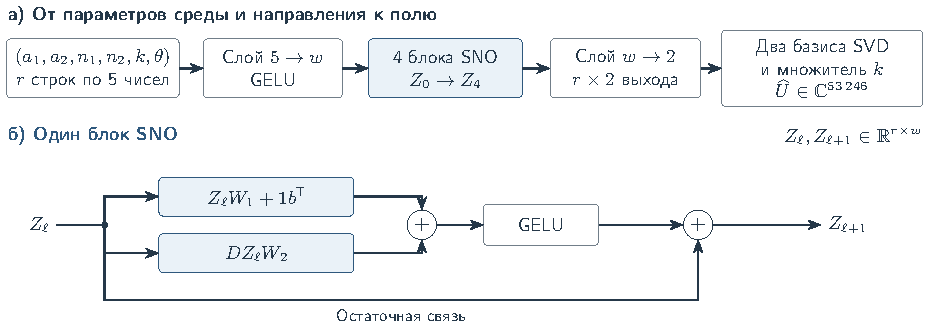
\includegraphics[width=.94\linewidth]{figures/architecture.pdf}
\captionof{figure}{Граф вычислений SVD-SNO. Вход содержит две пары материальных параметров, направление и волновое число. После последнего слоя коэффициенты двух компонент переводятся в узловое поле.}
\end{localfigure}
\clearpage
\section{Спектральные нейрооператоры}
\paragraph{SVD-SNO.}
Две группы материальных признаков и параметры волны подаются в таблицу мод. Первые две строки содержат стандартизованные $(a_j,n_j)$, далее материальные компоненты заполняются нулями. Волновое число и обе компоненты направления доступны каждой строке. В четырёх последовательных блоках вычисляется
\[
 Z'=Z+\operatorname{GELU}(ZW_1+\boldsymbol1 b^\T+DZW_2).
\]
Матрица $D$ связывает позиции мод, $W_1,W_2$ действуют по признакам. Выходной слой определяет коэффициенты действительной и мнимой частей. Их пространственное восстановление использует два базиса SVD.

\paragraph{Chebyshev-SNO и Fourier-SNO.}
В работе Фанаскова и Оселедца~\cite{fo} входные и выходные функции задаются конечными наборами спектральных коэффициентов. В настоящем опыте вход имеет конечную размерность: материал точно задан четырьмя скалярами, а падающая волна задана через $k$ и $\theta$. Скрытые слои преобразуют таблицу коэффициентов. Выход представляет две компоненты поля в тензорном базисе. Для $x=(x_1,x_2)$ чебышёвский базис состоит из произведений $T_j(x_1/2)T_l(x_2/2)$. Для Fourier-SNO используются вещественные косинусы $\cos(j\pi(x_1+2)/4)\cos(l\pi(x_2+2)/4)$, $0\le j,l<16$. Этот выбор соответствует чётному продолжению по каждой координате с периодом 8 и допускает различные значения на противоположных сторонах квадрата. Обе модели используют 256 коэффициентов на компоненту. Матрица $V$ содержит значения базиса в узлах; коэффициенты проекции решения определяются из $(V^\T M V)c=V^\T M f$. Семь параметрических признаков линейно переводятся в таблицу $16\times16$ с 24 каналами. В четырёх остаточных блоках обучаемые преобразования действуют по двум осям мод и по каналам, после чего применяется GELU. Такое построение адаптирует коэффициентный слой из приложения~C работы~\cite{fo} к непериодической задаче и треугольной сетке.


\paragraph{FNO.}
На прямоугольной сетке слой FNO вычисляет дискретное преобразование Фурье признаков, умножает сохранённые гармоники на обучаемые матрицы и выполняет обратное преобразование. Результат складывается с локальным линейным отображением перед применением нелинейности~\cite{li}. Использована равномерная сетка $32\times32$. Сеть получает координаты, четыре параметра среды, волновое число, компоненты направления, поля материалов и обе компоненты падающей волны. Последние признаки вычислены из тех же физических входных данных, что и у SNO. Если $T$ есть билинейное продолжение на узлы МКЭ, то матрица $T^\T MT$ задаёт норму выходной сетки. При обучении в функцию потерь включён также остаток проекции эталонного поля на это пространство.


\section{Вычислительная реализация}
По первым 124 точкам перемешанной семимерной последовательности Соболя заданы материалы и частоты. Четыре координаты определяют $p$. Три остальные задают по одному $k$ в каждой трети отрезка $[0{,}05;4]$. Для каждой среды дополнительно рассчитаны оба конца отрезка. При каждом из пяти $k$ используются направления $\theta=\pi/8$ и $5\pi/8$. Одной среде соответствуют десять полей. Начальное число генератора равно 20261124.

Первые 100 сред предназначены для обучения, следующие 12 для выбора параметров и ещё 12 для тестирования. Наборы из 400, 600, 800 и 1\,000 полей содержат соответственно 40, 60, 80 и 100 полных сред. Концы частотного диапазона и углы общие для всех выборок, внутренние частоты зависят от среды. Поэтому результаты на концах характеризуют перенос на другой материал, а внутри диапазона одновременно меняются материал и частота. Все методы оцениваются на одних и тех же узлах МКЭ после восстановления поля в исходном масштабе. \input{tables/budget}

\clearpage
\section{Численные эксперименты}
\subsection*{Объём выборки и разброс погрешности}
\begin{localtable}
\captionof{table}{Средняя относительная погрешность комплексного рассеянного поля на 120 тестовых задачах, \%. В заголовках указано число обучающих полей}
\begin{tabular}{lrrrr}\toprule Метод & 400 & 600 & 800 & 1\,000 \\\midrule
\tabinput{tables/size}\bottomrule\end{tabular}
\end{localtable}
\begin{localtable}
\captionof{table}{Результаты при 1\,000 обучающих полях. Приведены число обучаемых вещественных параметров $P$, валидационная погрешность и четыре тестовых характеристики, \%}
\begin{tabular}{lrrrrrr}\toprule Метод & $P$ & Валидация & Среднее & Медиана & $q_{0{,}95}$ & Максимум\\\midrule
\tabinput{tables/main}\bottomrule\end{tabular}
\end{localtable}

\begin{localfigure}
\includegraphics[width=.99\linewidth]{figures/errors.pdf}
\captionof{figure}{Средняя погрешность в зависимости от размера выборки и от волнового числа. Справа приведён результат при 1\,000 обучающих полях. Группы I, II и III относятся к внутренним частотам в трёх равных частях диапазона. Ось погрешности логарифмическая.}
\end{localfigure}
\begin{localtable}
\captionof{table}{Средняя погрешность в отдельных частотных группах, \%. В каждой ячейке учтены 12 сред и два направления}
\begin{tabular}{lrrrrr}\toprule Метод & $k=0{,}05$ & I & II & III & $k=4$\\\midrule
\tabinput{tables/band}\bottomrule\end{tabular}
\end{localtable}
\input{tables/comparison}

\clearpage
\subsection*{Погрешность вблизи нуля}
Чтобы проверить поведение моделей ниже нижней границы обучения, для первой тестовой среды дополнительно решены шесть задач. В табл.~\ref{tab:nearzero} приведены относительные ошибки по формуле~\eqref{eq:relative}. При каждом положительном $k$ знаменатель берётся по фактически рассчитанному полю. Нулевая абсолютная погрешность в статической точке следует из выбранной нормировки и множителя $k$ и сама по себе не гарантирует точности при сколь угодно малом положительном $k$.
\begin{localtable}
\captionof{table}{Экстраполяция при $k<0{,}05$. Средняя относительная погрешность двух направлений при 1\,000 обучающих полях, \%}\label{tab:nearzero}
\begin{tabular}{lrrr}\toprule Метод & $0{,}001$ & $0{,}01$ & $0{,}025$\\\midrule
\tabinput{tables/nearzero}\bottomrule\end{tabular}
\end{localtable}
\input{tables/near_note}

\subsection*{Абсолютная погрешность и различия между средами}
Дополнительно вычислим абсолютную величину $\norm{\widehat U-U_h}_M$ и для каждой из 12 тестовых сред усредним относительную погрешность по её десяти полям. Таким образом, можно сравнить разброс между средами при одинаковом числе наблюдений на среду. В табл.~\ref{tab:absolute} входят только положительные частоты основного теста.
\begin{localtable}
\captionof{table}{Абсолютная $L^2$-погрешность и диапазон средних относительных погрешностей по средам при 1\,000 обучающих полях}\label{tab:absolute}
\begin{tabular}{lrrr}\toprule Метод & Средняя абсолютная & Мин. по средам, \% & Макс. по средам, \%\\\midrule
\tabinput{tables/absolute}\bottomrule\end{tabular}
\end{localtable}
\clearpage
\subsection*{Выбор числа мод и числа параметров}
В SVD-SNO увеличение ранга расширяет пространство, в котором восстанавливается поле, и одновременно увеличивает размер матрицы связей $D$ в каждом из четырёх блоков. В таблице ниже $r$ есть число мод для одной вещественной компоненты. Лучший ранг выбирался отдельно по каждому столбцу. Размер базиса, построенного по снимкам, не входит в число обучаемых весов $P$.
\begin{localtable}
\captionof{table}{Валидационная погрешность SVD-SNO, \%, для трёх рангов и четырёх объёмов обучения. Полужирным отмечен выбранный ранг}
\begin{tabular}{rrrrrr}\toprule $r$ & $P$ & 400 & 600 & 800 & 1\,000 \\\midrule
\tabinput{tables/ranks}\bottomrule\end{tabular}
\end{localtable}
У Chebyshev-SNO и Fourier-SNO число мод совпадает по построению. Чтобы оценить, какую часть погрешности вносит выбор базиса, для каждого тестового решения можно вычислить его ортогональную проекцию, используя само решение. Средние остатки этих проекций равны $3{,}90\%$ для полиномов Чебышёва и $3{,}55\%$ для косинусов. Эти величины задают достижимую нижнюю границу погрешности при произвольном выборе коэффициентов в соответствующем пространстве. В FNO удержанные моды относятся к преобразованию внутри слоя; число степеней свободы выходного поля определяется узлами прямоугольной сетки.
\subsection*{Сравнение с GMsFEM}
Для каждой тестовой среды строилось пространство GMsFEM~\cite{gms} типа~I на сетке из 17\,549 узлов. Квадрат разделён на $20\times20$ крупных ячеек. В окрестности каждой крупной вершины вычислялись $a$-гармонические продолжения граничных следов. После решения локальной спектральной задачи сохранялись первые $m$ моды, умноженные на функции разбиения единицы. Базис одной среды повторно использовался для пяти частот. При каждой частоте решалась комплексная система Галёркина для двух правых частей. Результат переносился на эталонную сетку и сравнивался с теми же 120 решениями.
\begin{localtable}
\captionof{table}{Погрешность GMsFEM на общем тесте, \%. Размер системы указан в комплексных неизвестных}
\begin{tabular}{rrrrr}\toprule $m$ & Размер & Среднее & $q_{0{,}95}$ & При $k=4$\\\midrule
\tabinput{tables/gms}\bottomrule\end{tabular}
\end{localtable}
\input{tables/gms_note}
\clearpage
\subsection*{Пространственное распределение поля}
Для качественного сравнения выбрана первая тестовая среда при $k=4$, $\theta=\pi/8$. Этот выбор фиксирован по номеру задачи. Верхний ряд рис.~\ref{fig:fields} показывает амплитуду рассеянного поля. В нижнем ряду изображён модуль разности комплексных полей. Поэтому в картах ошибки учитывается расхождение фаз даже там, где амплитуды визуально близки.
\begin{localfigure}
\includegraphics[width=\linewidth]{figures/fields.pdf}
\captionof{figure}{Рассеянное поле МКЭ и прогнозы четырёх моделей на общей треугольной сетке. Внутри каждого ряда используется одна цветовая шкала.}
\label{fig:fields}
\end{localfigure}
\input{tables/example}
\section{Заключение}
\input{tables/conclusion}
Выводы относятся к двум группам изотропных материалов, двум направлениям падающей волны и одной геометрии. Оценки по 120 полям включают группы по десять полей одной среды. Разброс при повторной инициализации сети и погрешность замены внешней задачи поглощающим условием в этот опыт не входят.

\begingroup\small\begin{thebibliography}{9}\setlength{\itemsep}{0pt}
\bibitem{fo} Fanaskov V., Oseledets I. Spectral Neural Operators. Авторская версия \href{https://arxiv.org/abs/2205.10573}{arXiv:2205.10573}, приложение C.
\bibitem{li} Li Z., Kovachki N., Azizzadenesheli K. et al. Fourier Neural Operator for Parametric Partial Differential Equations. \emph{International Conference on Learning Representations}. 2021. \href{https://arxiv.org/abs/2010.08895}{arXiv:2010.08895}.
\bibitem{gms} Efendiev Y., Galvis J., Hou T. Y. Generalized multiscale finite element methods (GMsFEM). \emph{Journal of Computational Physics}. 2013. Vol.~251. P.~116--135. \href{https://doi.org/10.1016/j.jcp.2013.04.045}{DOI:10.1016/j.jcp.2013.04.045}.
\bibitem{sirovich} Sirovich L. Turbulence and the dynamics of coherent structures. Part I. Coherent structures. \emph{Quart. Appl. Math.} 1987. Vol.~45. P.~561--571.
\end{thebibliography}\endgroup
\end{document}
